\section{Numerical solutions}
In this section we numerically solve the linear stability problem
corresponding to Eq. \ref{lin_mass}---\ref{lin_energy}. 
We relax the thin-disk, low-frequency and nearly-Keplerian
approximations used in the discussion above, and 
use the full, non-Keplerian expressions of $\rho$, $\Omega$ and
$\kappa$, so that we may consider vertical domains up to $z\sim r$.  

% \subsection{Boundary conditions}
% In numerical calculations a finite vertical domain $z\in[-1,1]\zmax$
% is adopted. For $\Gamma\neq1$ we take $\zmax$ to be slightly less than
% $H$ to avoid the zero-density surface. At $z=\pm\zmax$ we impose
% \begin{align}
%   \delta v_z = 0,
% \end{align}
% for a solid boundary, or 
% \begin{align}
%   \Delta P \equiv \delta P + \bm{\xi}\cdot\nabla P= 0,  
% \end{align}
% for a free surface, where $\bm{\xi}$ is the Lagrangian
% displacement.

We solve the linear problem by expanding the
perturbations in Chebyshev polynomials $T_l$ up to $l=512$
and discretizing the equations on a grid with
$z\in[-\zmax,\zmax]$. At the vertical boundaries we impose a free
surface, 
\begin{align}
  \Delta P \equiv \delta P + \bm{\xi}\cdot\nabla P= 0 \quad \text{at } z=\pm\zmax,
\end{align}
where $\bm{\xi}$ is the Lagrangian displacement. This boundary
condition was found to be most convenient for numerical
implementation. The above discretization procedure converts the linear  
system of differential equations to a standard matrix eigenvalue
problem.     

Unless otherwise stated, our fiducial disk model is a
nearly-vertically isothermal disk with $\Gamma=1.011$, $p=-1.5$,
$q=-1$, $\epsilon=0.1$, $\zmax = 10\epsilon r$, and the perturbation
wavenumber $k_x = 200\pi/r$ (or $\hat{k}=20\pi$). 


\subsection{VSI in a neutrally stratified disk}\label{vertiso_pertiso} 
We first test our numerical code, as well as the discussion in
\S\ref{iso_discuss}, by considering nearly-isothermal
perturbations. We set $\gamma=1.011=\Gamma$, and effectively switch
off thermal relaxation by choosing $\beta=10^9$. The vertical domain is
$\zmax = 10\epsilon r$. This setup is very similar to that adopted in
\cite{mcnally14}, who calculated the VSI in vertically isothermal
disks subject to isothermal perturbations ($\Gamma=\gamma=1$).  


Fig. \ref{lowfreq_eigen} shows the eigenvalues $\sigma = \omega +
\ii\nu$. This plot is effectively identical to that in
\cite{mcnally14}. The fundamental VSI mode, with one node in $W$, has
the smallest $|\sigma|$ and is shown in Fig. \ref{lowfreq_eigenfunc}.  
Its expected growth rate, calculated from Eq. \ref{simple_growth} with  
$L=1$, and the numerically-obtained value are 
\begin{align*}
  \nu = 0.2606\epsilon\Omega_k &\quad \text{(from
    Eq. \ref{simple_growth})},\\
  \nu = 0.2577 \epsilon \Omega_k &\quad \text{(numerical)}.
\end{align*}
This agreement is surpsingly good, given that
Eq. \ref{simple_growth} assumes a thin, nearly-Keplerian disk in the 
low-frequency approximation, and
imposes a different boundary condition to that in the numerical
calculation. The eigenfrequency is not very sensitive to the vertical boundary
condition because the expression for $\sigma$, given by
Eq. \ref{integral_relation1}, involve integrands with $\rho$ as the 
weight function, which rapidly decays away from the midplane. The
eigenfunction $W$ is qualitatively proportional to 
$z$, as expected for the fundamental mode according to explicit
solutions discussed in \S\ref{iso_poly}.    

\begin{figure}
  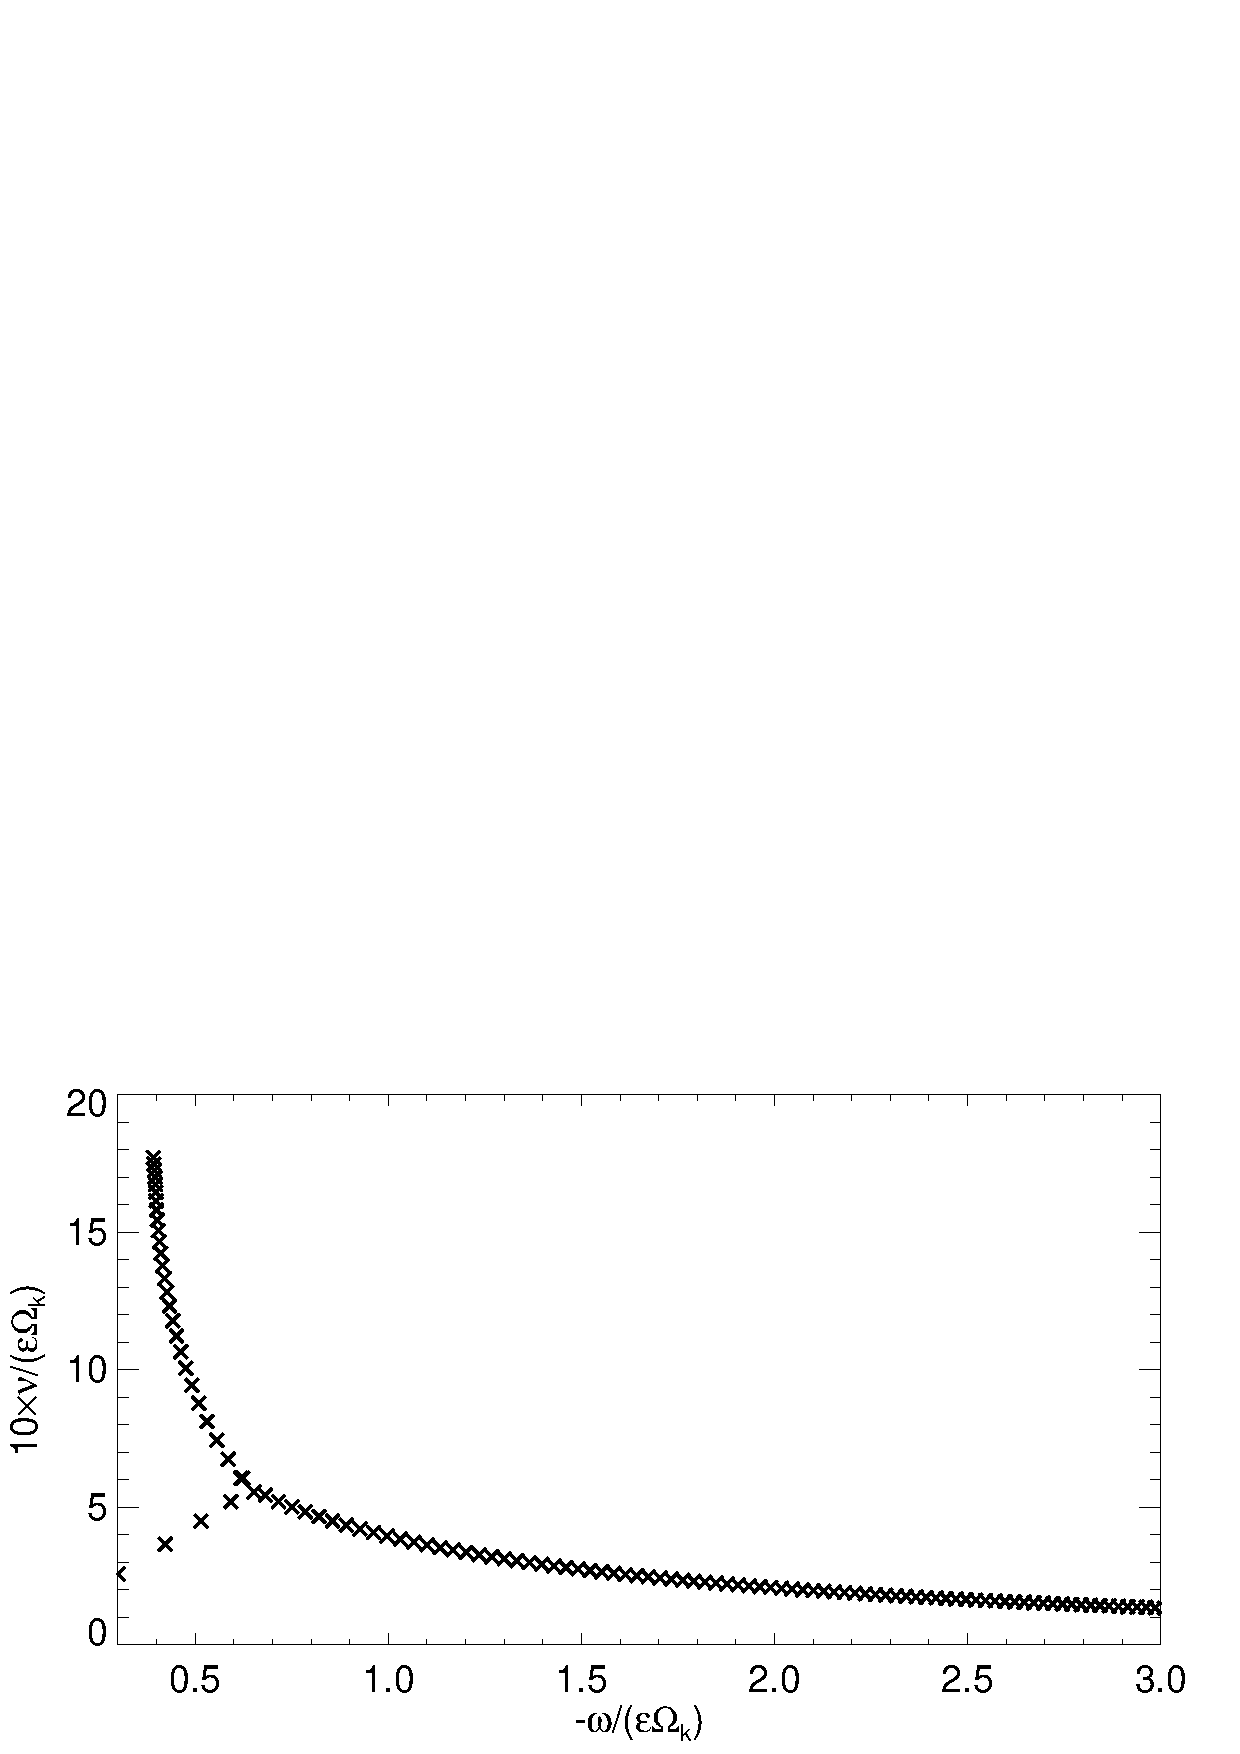
\includegraphics[width=\linewidth]{figures/eigenvalues_iso}
  \caption{Eigenvalues of the
    vertical shear instability in a neutrally-stratified,
    nearly-vertically isothermal disk  ($\gamma=\Gamma=1.011$). The
    disk parameters are $q=-1$,  
    $p=-1.5$ and $\epsilon=0.1$, while the perturbation radial
    wavenumber is $k_x=200\pi/r$. This is the set up considered in
    \cite{mcnally14}. \label{lowfreq_eigen}
  }
\end{figure}

\begin{figure}
  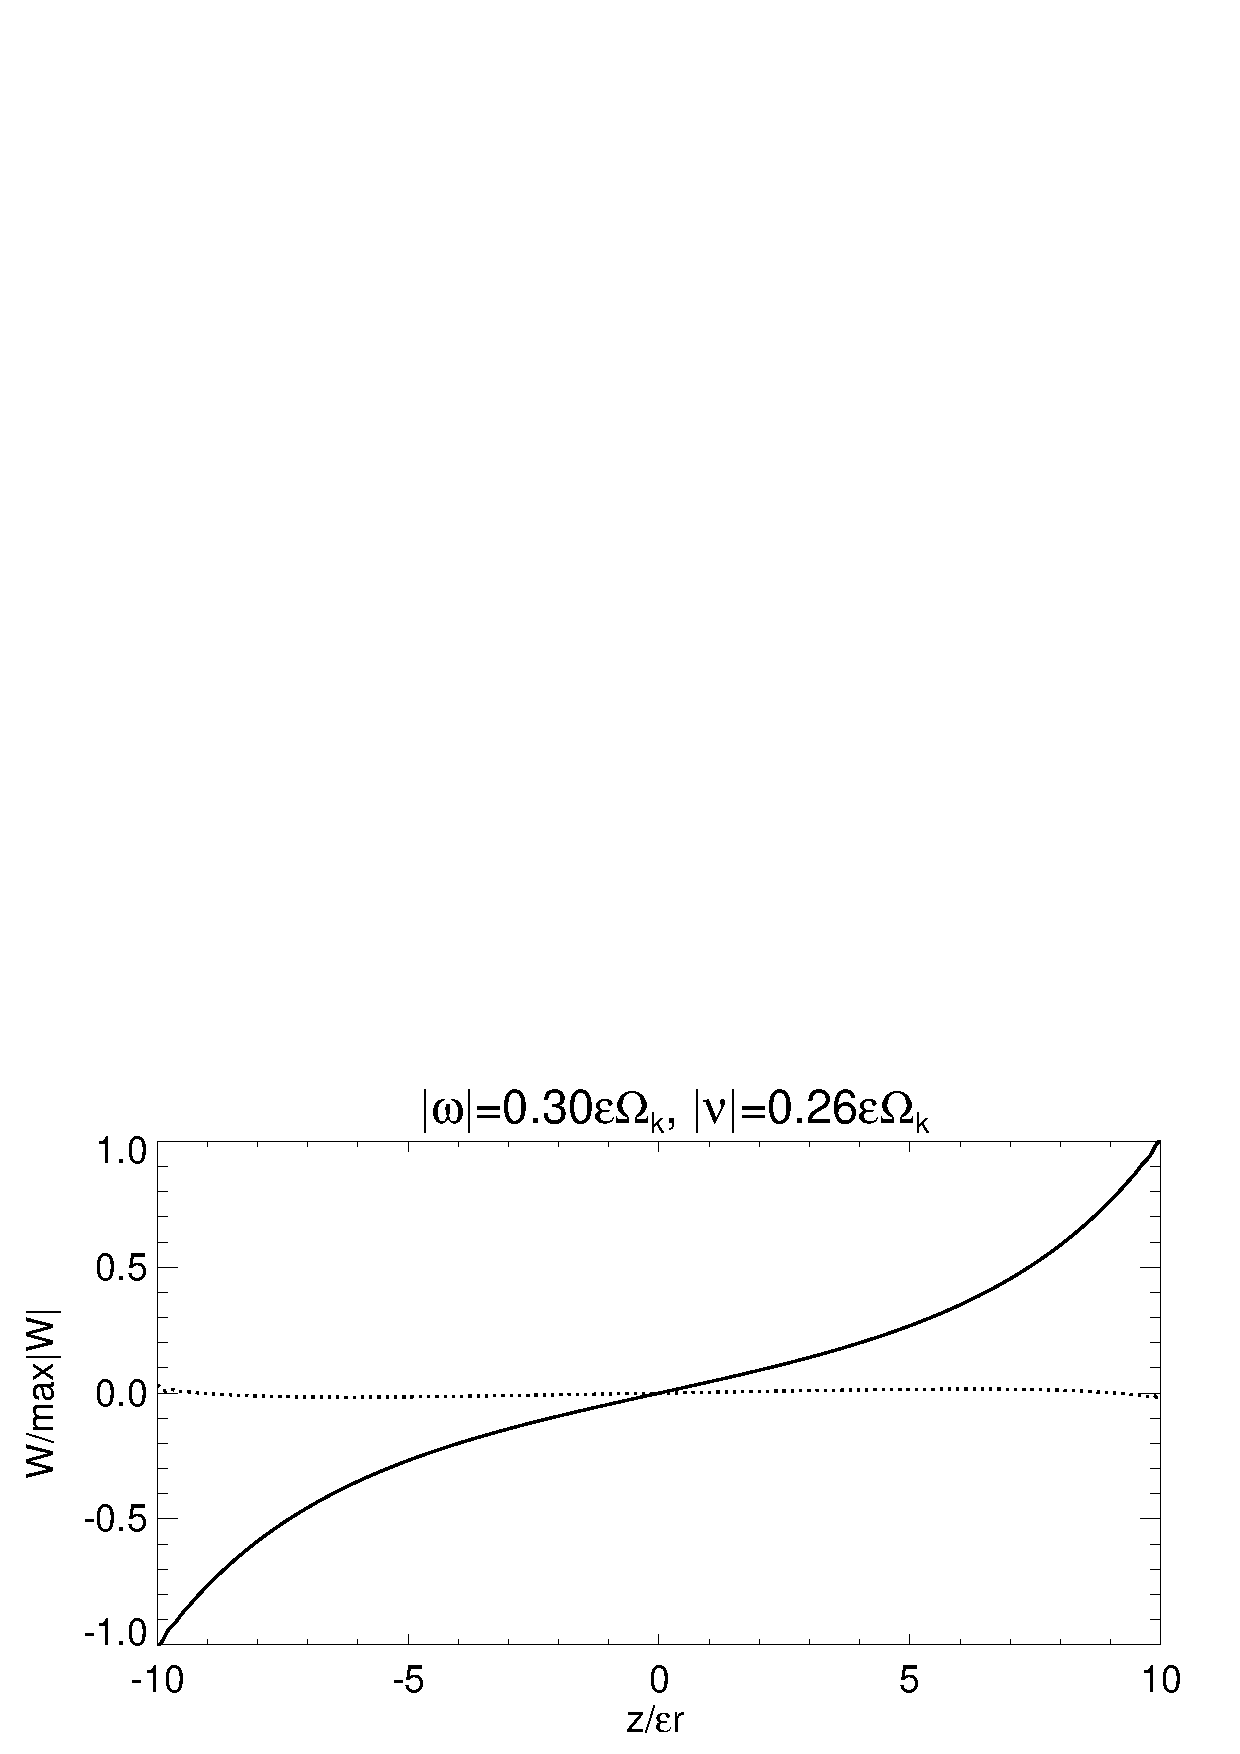
\includegraphics[width=\linewidth]{figures/eigenvector_iso}
  \caption{Eigenfunction of the fundamental VSI,
    corresponding to the bottom-left eigenvalue displayed in
    Fig. \ref{lowfreq_eigen} (smallest $|\sigma|$). The
    solid and dashed lines are $\real W$ and $\imag W$, respectively. 
    \label{lowfreq_eigenfunc}
  }
\end{figure}

% We have also solved this problem with in the low-frequency 
% approximation by setting $D\to\kappa^2$ in Eq. \ref{ode_w} (with $Q=W$). We
% obtained very similar results, as expected for modes with
% $|\sigma/\Omega_k|\ll1$. 

\subsection{Stabilization of the VSI by a positive vertical entropy
  gradient}
We demonstrate the (strong) stabilizing effect of a  
positive vertical entropy gradient by setting $\gamma=2$.  
Since we expect the perturbations to decay rapidly
away from the midplane (see \S\ref{analytic_adia}), we consider a
smaller domain with $\zmax = 2\epsilon r$. 
Other disk and perturbation parameters are the same as in
\S\ref{vertiso_pertiso}.    

% We use the same pseudo-spectral method as before. Here we set
% $\zmax = 2\epsilon r$ and impose a free surface. This boundary
% condition was found to be most convenient for numerical
% implementation. Since we expect the perturbations to decay rapidly
% away from the midplane (see \S\ref{analytic_adia}), we do not expect 
% boundary conditions to play an important role, provided that $\zmax$ is
% sufficiently large. 

Fig. \ref{lowfreq_eigen_adia} show the eigenvalues for this
problem. The growth rates are about an order of magnitude smaller than
the previous case. The fundamental VSI mode is that with
$\mathrm{max}|\nu|$. Its expected and numerically-calculated growth
rates compares well, with 
\begin{align*}
  \nu = 0.03751 \epsilon \Omega_k &\quad \text{(from
    Eq. \ref{gam2_growth_rate})},\\
  \nu = 0.03672 \epsilon \Omega_k &\quad \text{(numerical)}.
\end{align*}
The fundamental mode is plotted in Fig. \ref{lowfreq_eigenfunc_adia},
and clearly show that perturbations are rapidly stabilized away from
the midplane. For the adopted disk and perturbation parameters 
($|q|=1$ and $\hat{k} = 20\pi$), Eq. \ref{gam2_alpha} gives $\real{\alpha}\simeq - 43.8$,
corresponding to a characteristic decay length scale of $\simeq
0.15\epsilon r$, which is consistent with that observed in 
Fig. \ref{lowfreq_eigenfunc_adia}. 

Coincidentally, this decay lengthscale is rougly the height within which
vertical shear is larger than the buoyancy frequency squared. That is,
\begin{align*}
\left|r\frac{d\Omega^2}{dz}\right|\gtrsim N_z^2
\end{align*}
for
\begin{align*}
  \left|\frac{z}{\epsilon r}\right| \lesssim \frac{\epsilon|q|\gamma}{\gamma-1},
\end{align*}
in a thin, vertically isothermal disk. This evaluates to $z\sim
0.2\epsilon r$ for the current disk model, consistent with
Fig. \ref{lowfreq_eigenfunc_adia}. 

Furthermore, the growth rate to should be no larger than the
maximum vertical shear available within this decay lengthscale. Using 
Eq. \ref{max_growth} as a rough guide, 
\begin{align}
  \frac{\nu}{\epsilon\Omega_k}<\frac{\epsilon |q|^2\gamma}{2(\gamma-1)},
\end{align}
or $\nu< 0.1\epsilon\Omega_k$ is expected in our disk model,
consistent with numerical results. 


\begin{figure}
  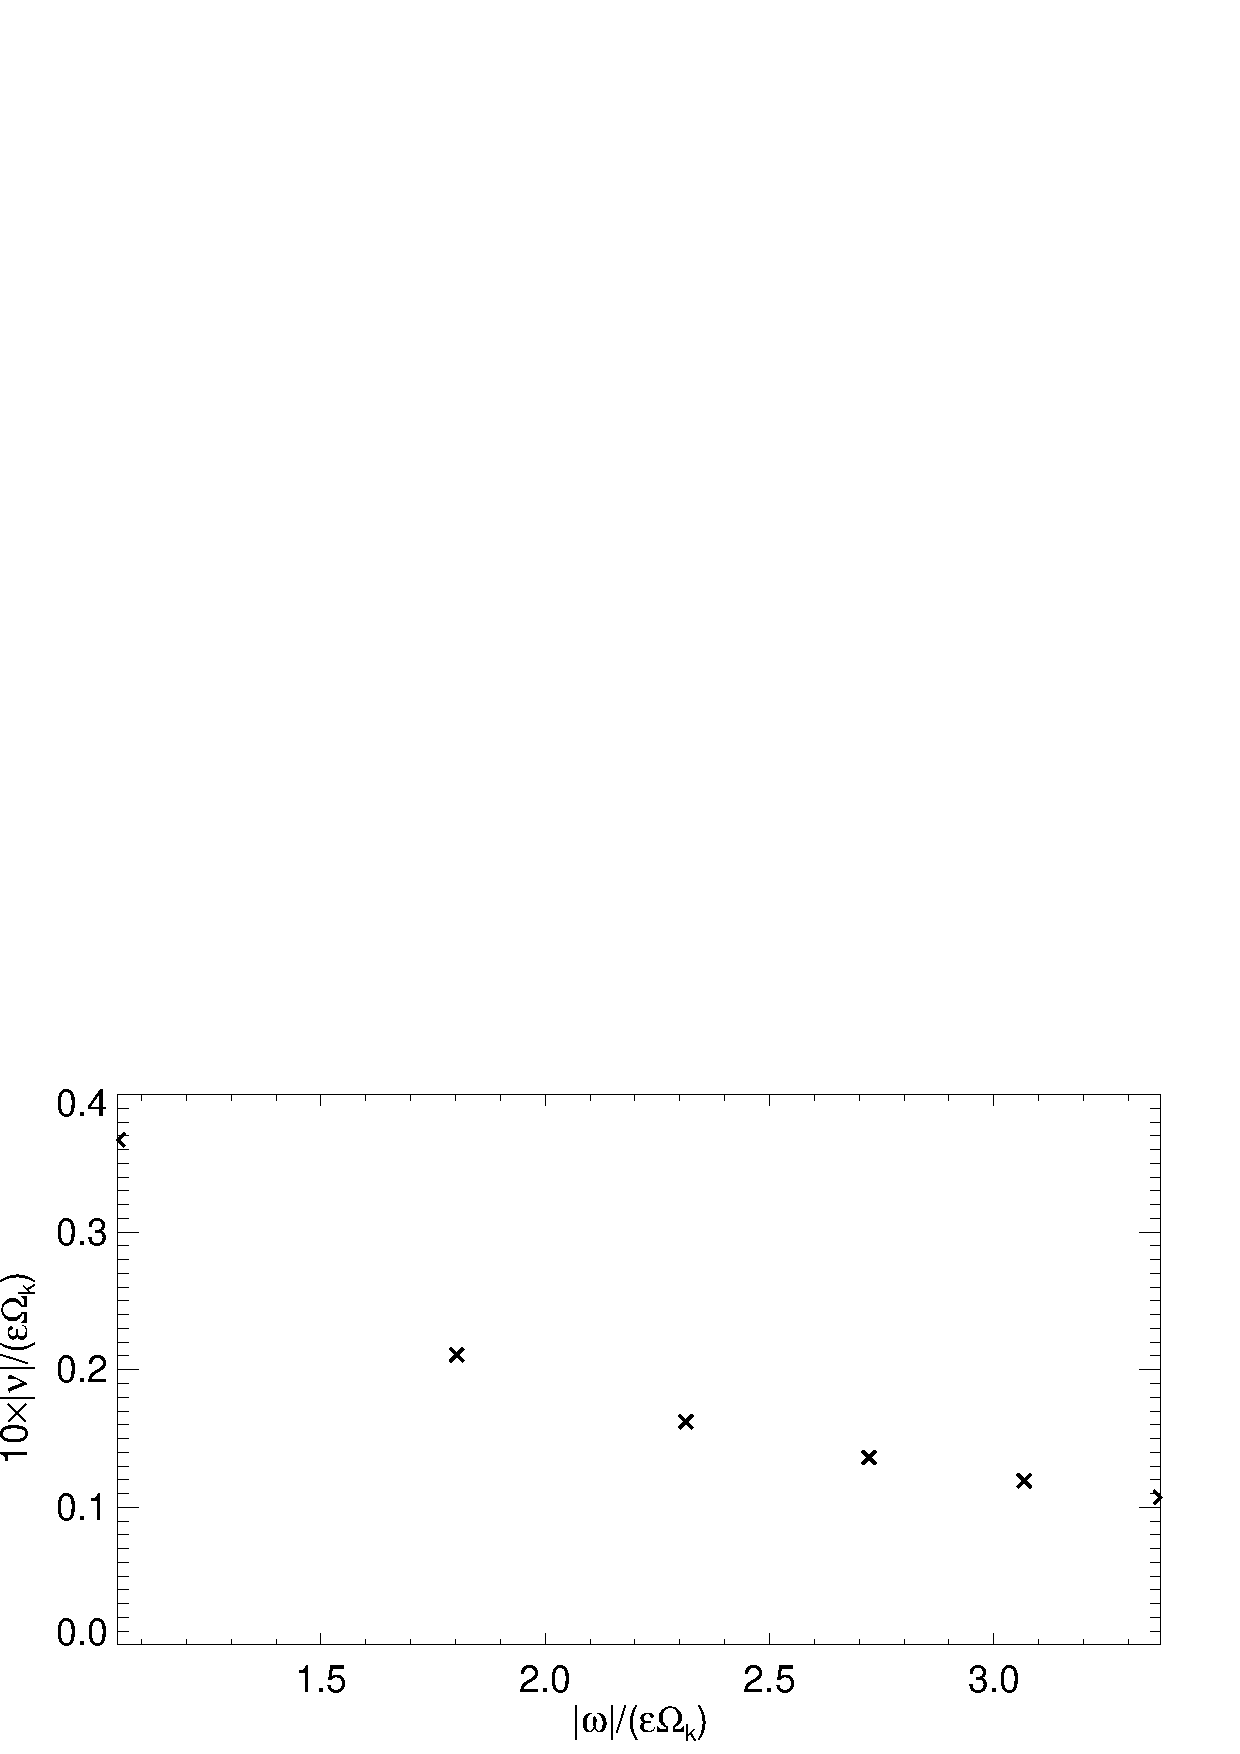
\includegraphics[width=\linewidth]{figures/eigenvalues_adia}
  \caption{Eigenvalues in for the
    vertical shear instability in a nearly-vertically isothermal disk
    ($\Gamma=1.011$) evolved adiabatically with $\gamma=2$ and
    $\beta=10^9$. The disk
    parameters are $q=-1$, 
    $p=-1.5$ and $\epsilon=0.1$, while the perturbation radial
    wavenumber is $k_x=200\pi/r$. \label{lowfreq_eigen_adia}
  }
\end{figure}
  

\begin{figure}
  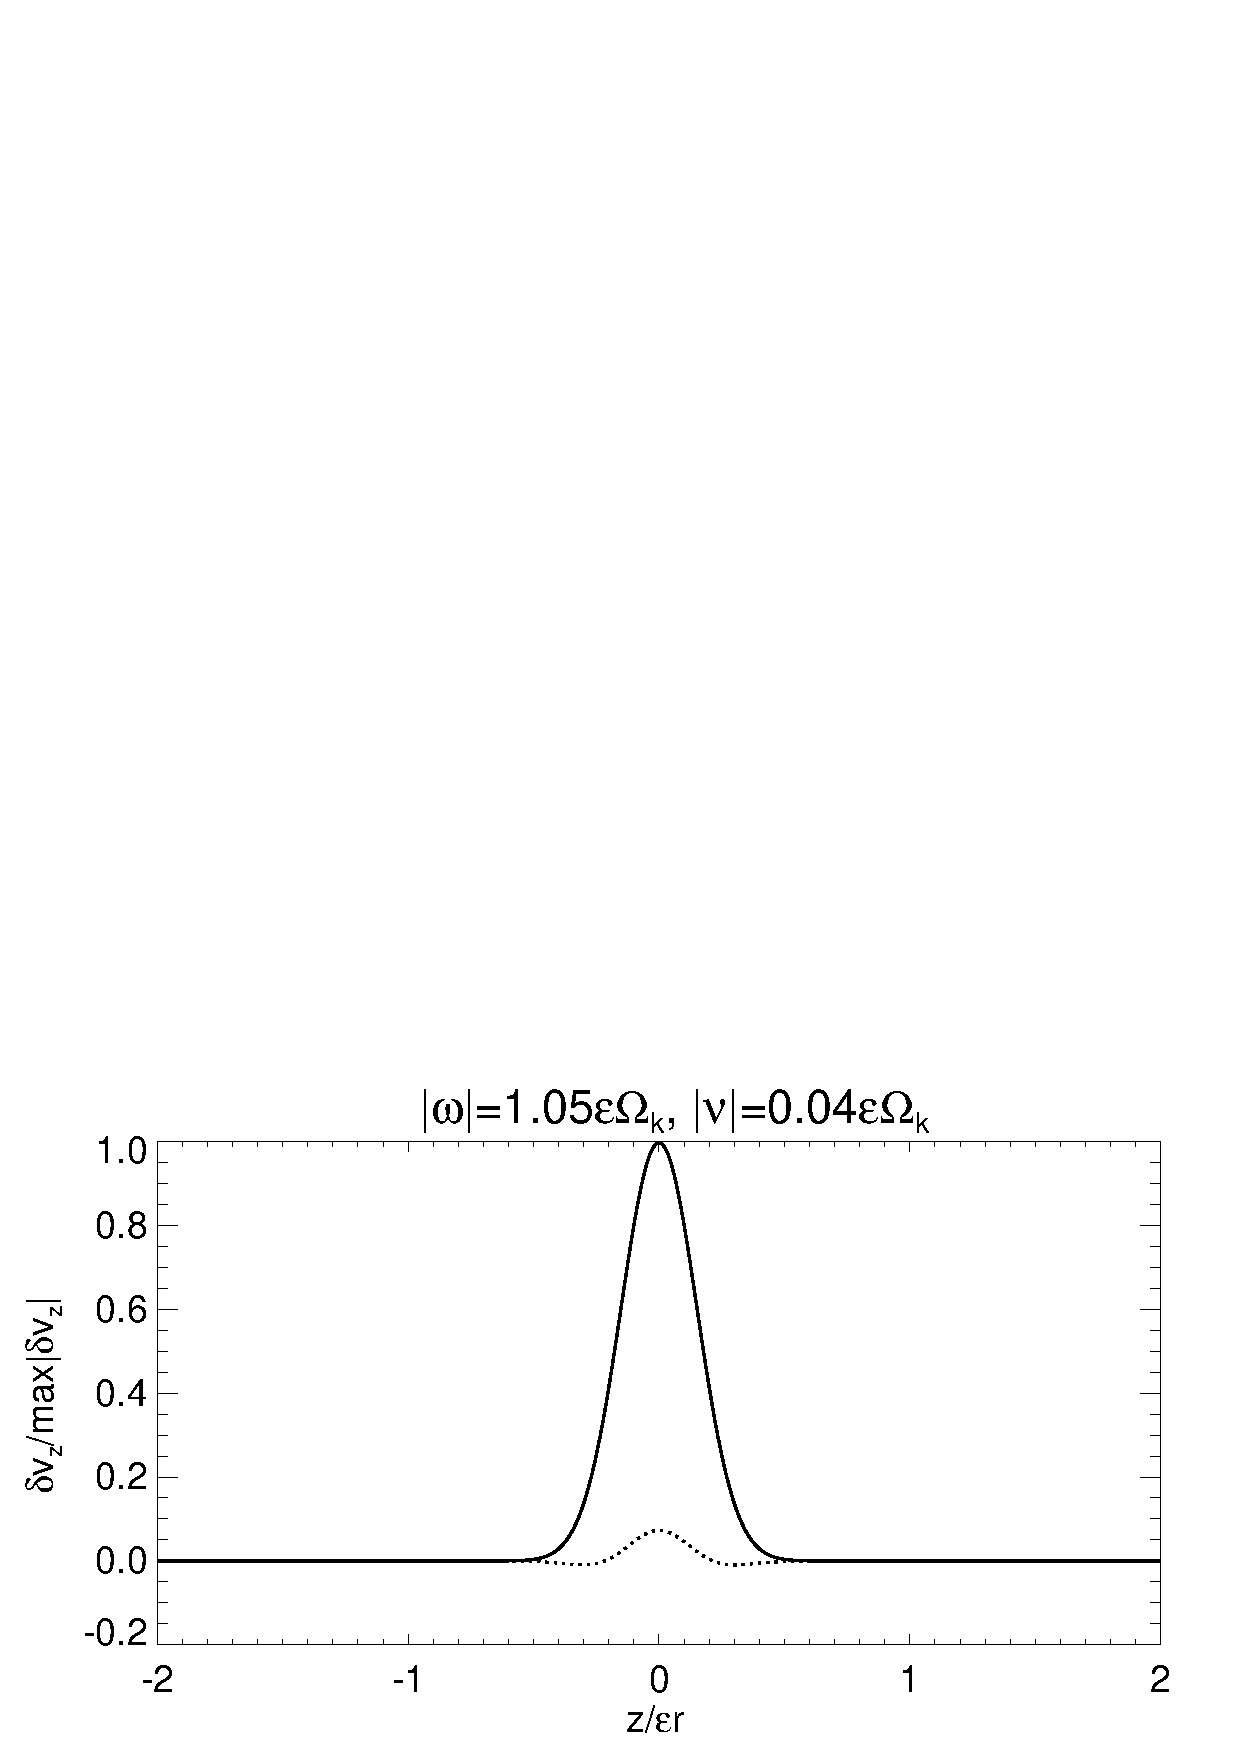
\includegraphics[width=\linewidth]{figures/eigenvectorvz_adia}
  \caption{Fundamental VSI mode in a nearly-vertically
    isothermal disk ($\Gamma=1.011$) evolved adiabatically
    ($\gamma=2$, $\beta=10^9$). This eigenfunction 
    corresponds to the top-left eigenvalue displayed in 
    Fig. \ref{lowfreq_eigen_adia} (largest $|\nu|$).  
    The solid and dashed lines are $\real \delta v_z$ and $\imag
    \delta v_z$, respectively.  
    \label{lowfreq_eigenfunc_adia}
  }
\end{figure}


% We have also solved this problem in the low-frequency approximation
% using Eq. \ref{ode_w}---\ref{ode_Q} with the replacement
% $D\to\kappa^2$. We again obtained very similar results. 


\subsection{Other adiabatic indices}
In Fig. \ref{adia_growth_num} we plot the eigenfrequencies of the
fundamental VSI mode for $\gamma\in[1,2]$. To select the appropriate
eigenvalues we vary the parameters slowly away from a reference solution.   

% The numerically-determined eigenfrequencies are qualitatively
% consistent with the discussion in \S\ref{adia_compare_gam1}.
There is good agreement between Fig. \ref{adia_growth_num} and
Fig. \ref{adia_growth} for $k_xH_\mathrm{iso}\gtrsim10$. There is a
mistach for smaller wavenumbers, especially in the growth
rates. Actual growth rates decrease slower as $k_xH_\mathrm{iso}\to0$
than that in Fig. \ref{adia_growth}. Disagreement at small
$k_xH_\mathrm{iso}$ is not surprising because the low-frequency
approximation used to obtain Fig. \ref{adia_growth} becomes invalid since
$|\omega|\sim\Omega_k$ for small $k_x$. 

Given the number of approximations made in \S\ref{adia_compare_gam1},
Fig. \ref{adia_growth_num} compares well with
Fig. \ref{adia_growth}. The main qualitative features of the full
numerical solution in Fig. \ref{adia_growth_num} are captured by
Fig. \ref{adia_growth}: stabilization for
$k_xH_\mathrm{iso}\to0$ and $k_xH_\mathrm{iso}\to\infty$,
stabilization for increasing $\gamma$ (but ineffective at small $k_x$), 
and the shift of the most unstable wavenumber to smaller values as
$\gamma$ is increased. 


\begin{figure}
  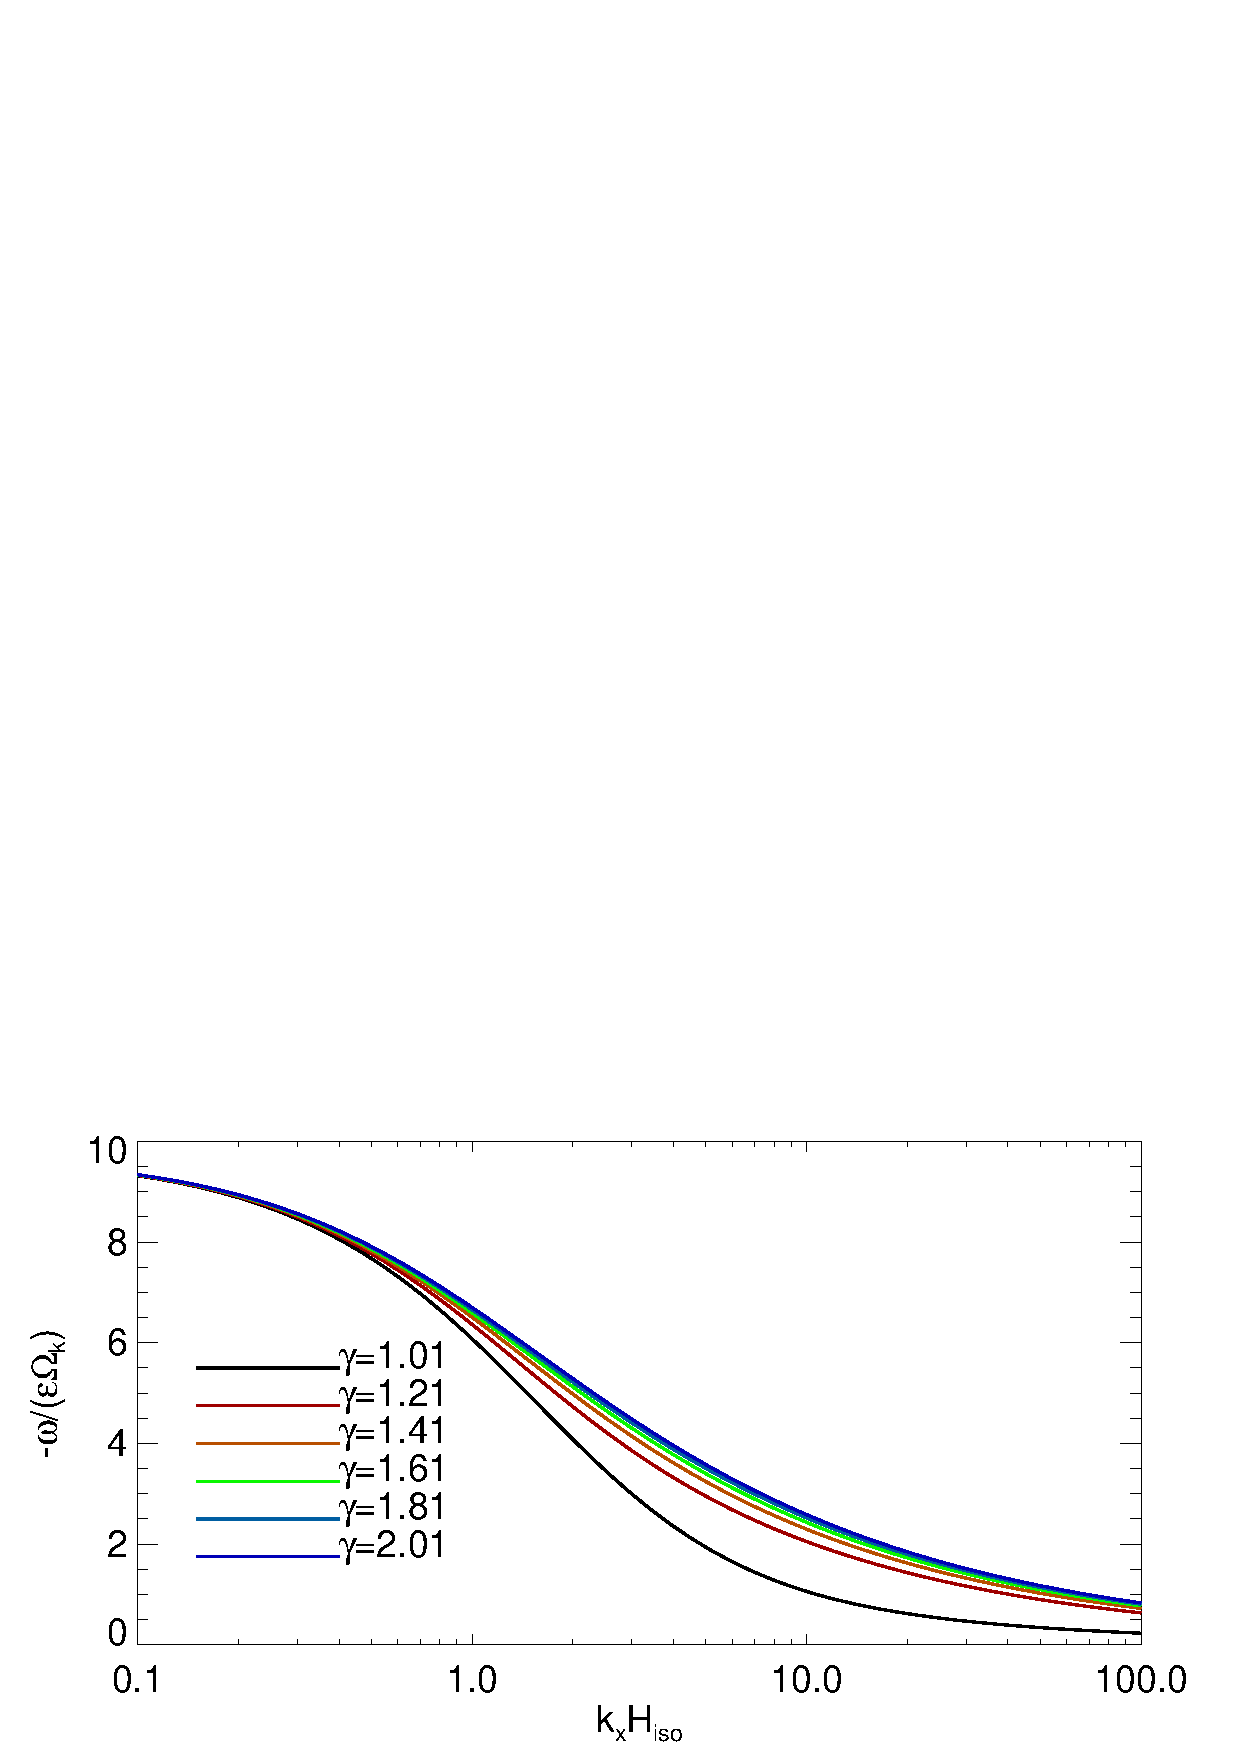
\includegraphics[width=\linewidth,clip=true,trim=0cm 1.75cm 0cm 0cm]{figures/compare_eigen_real1}
  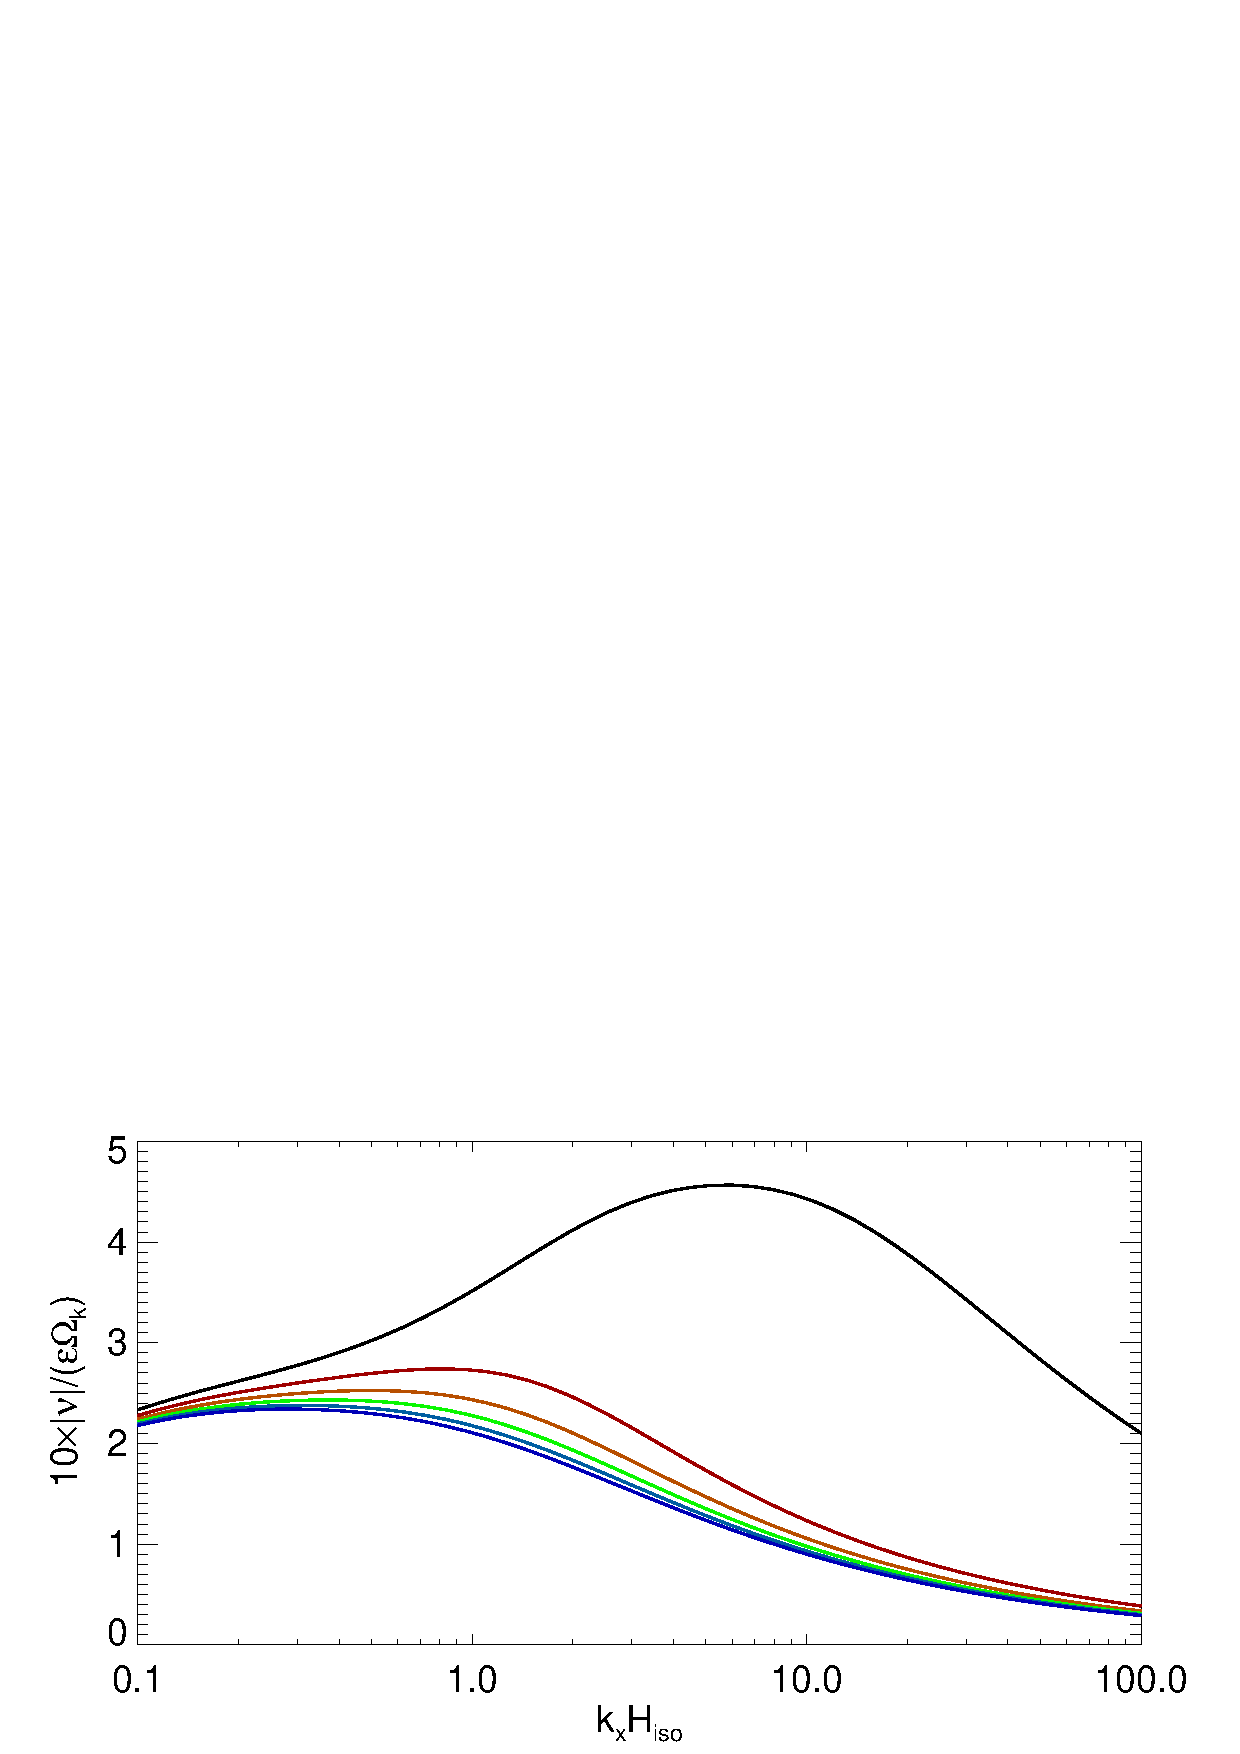
\includegraphics[width=\linewidth,clip=true,trim=0cm 0cm 0cm 1cm]{figures/compare_eigen_imag1}
  \caption{Real frequency (top) and growth rate 
    (bottom) of the fundamental VSI mode in nearly-vertically   
    isothermal disks ($\Gamma=1.011$) with $\epsilon=0.1$ and  
    $q=-1$, subject to adiabatic perturbations
    ($\beta=10^9$). The eigenfrequencies are calculated by numerically
    solving the full linear eigenvalue problem. This plot is to
    be compared with Fig. \ref{adia_growth}. \label{adia_growth_num}}   
\end{figure}   

\subsection{Effect of thermal relaxation}
We now introduce thermal relaxation. Here we consider a slightly
different disk model with $\epsilon=0.05$ and $\gamma=1.4$, as
adopted in \cite{nelson13}. Fig. \ref{relax_growth_num} plots the
growth rates of the fundamental mode function of $k_x$. %corrugation
                                %mode 
% We first obtain the eigenvalues for the
% fundamental mode for $k_xH_\mathrm{iso}=0$, then vary parameters
% slowly to obtain eigenvalues for other values of $k_x$ or $\beta$.   

As above, Fig. \ref{relax_growth_num} is largely consistent with 
Fig. \ref{relax_disp_fig} except for $k_xH_\mathrm{iso}\lesssim 1$
where the low-frequency approximation fails. The non-smoothness in the
curve for $\beta=0.063$ at $k_xH_\mathrm{iso}\sim50$ was found to be
associated with large perturbations near the vertical boundaries. This is
likely attributable to the free surface boundary condition imposed in
the numerical calculation (cf. regularity condition at infinity in
\S\ref{disp_relax}).    

Fig. \ref{relax_growth_num} confirms our analytical discussion that
introducing a small but finite cooling time stabilizes the fundamental
VSI, but there is a preferable wavenumber around $k_xH_\mathrm{iso} =
O(10)$ that maximizes this effect. 

\begin{figure}
   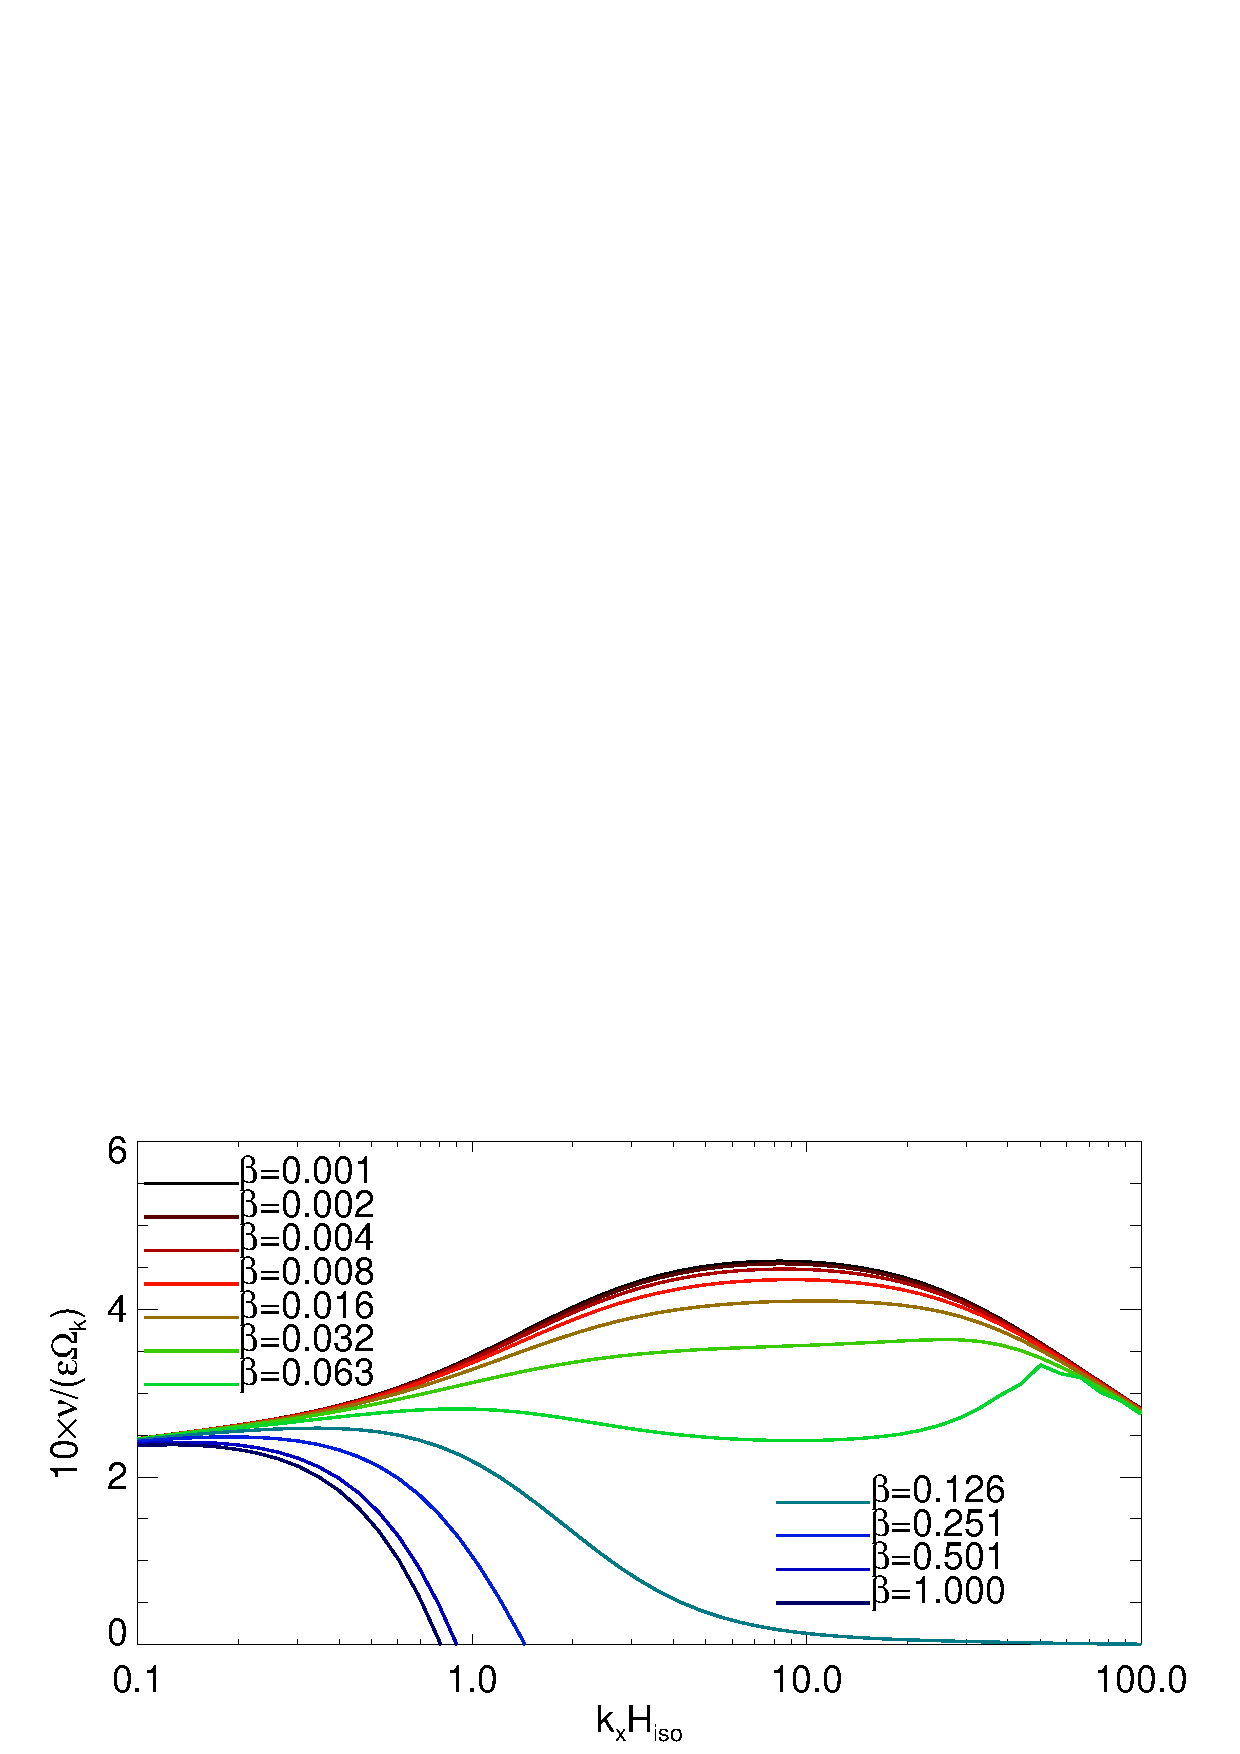
\includegraphics[width=\linewidth,clip=true,trim=0cm 1.75cm 0cm 0cm]{figures/compare_eigen_imag_bloop}
  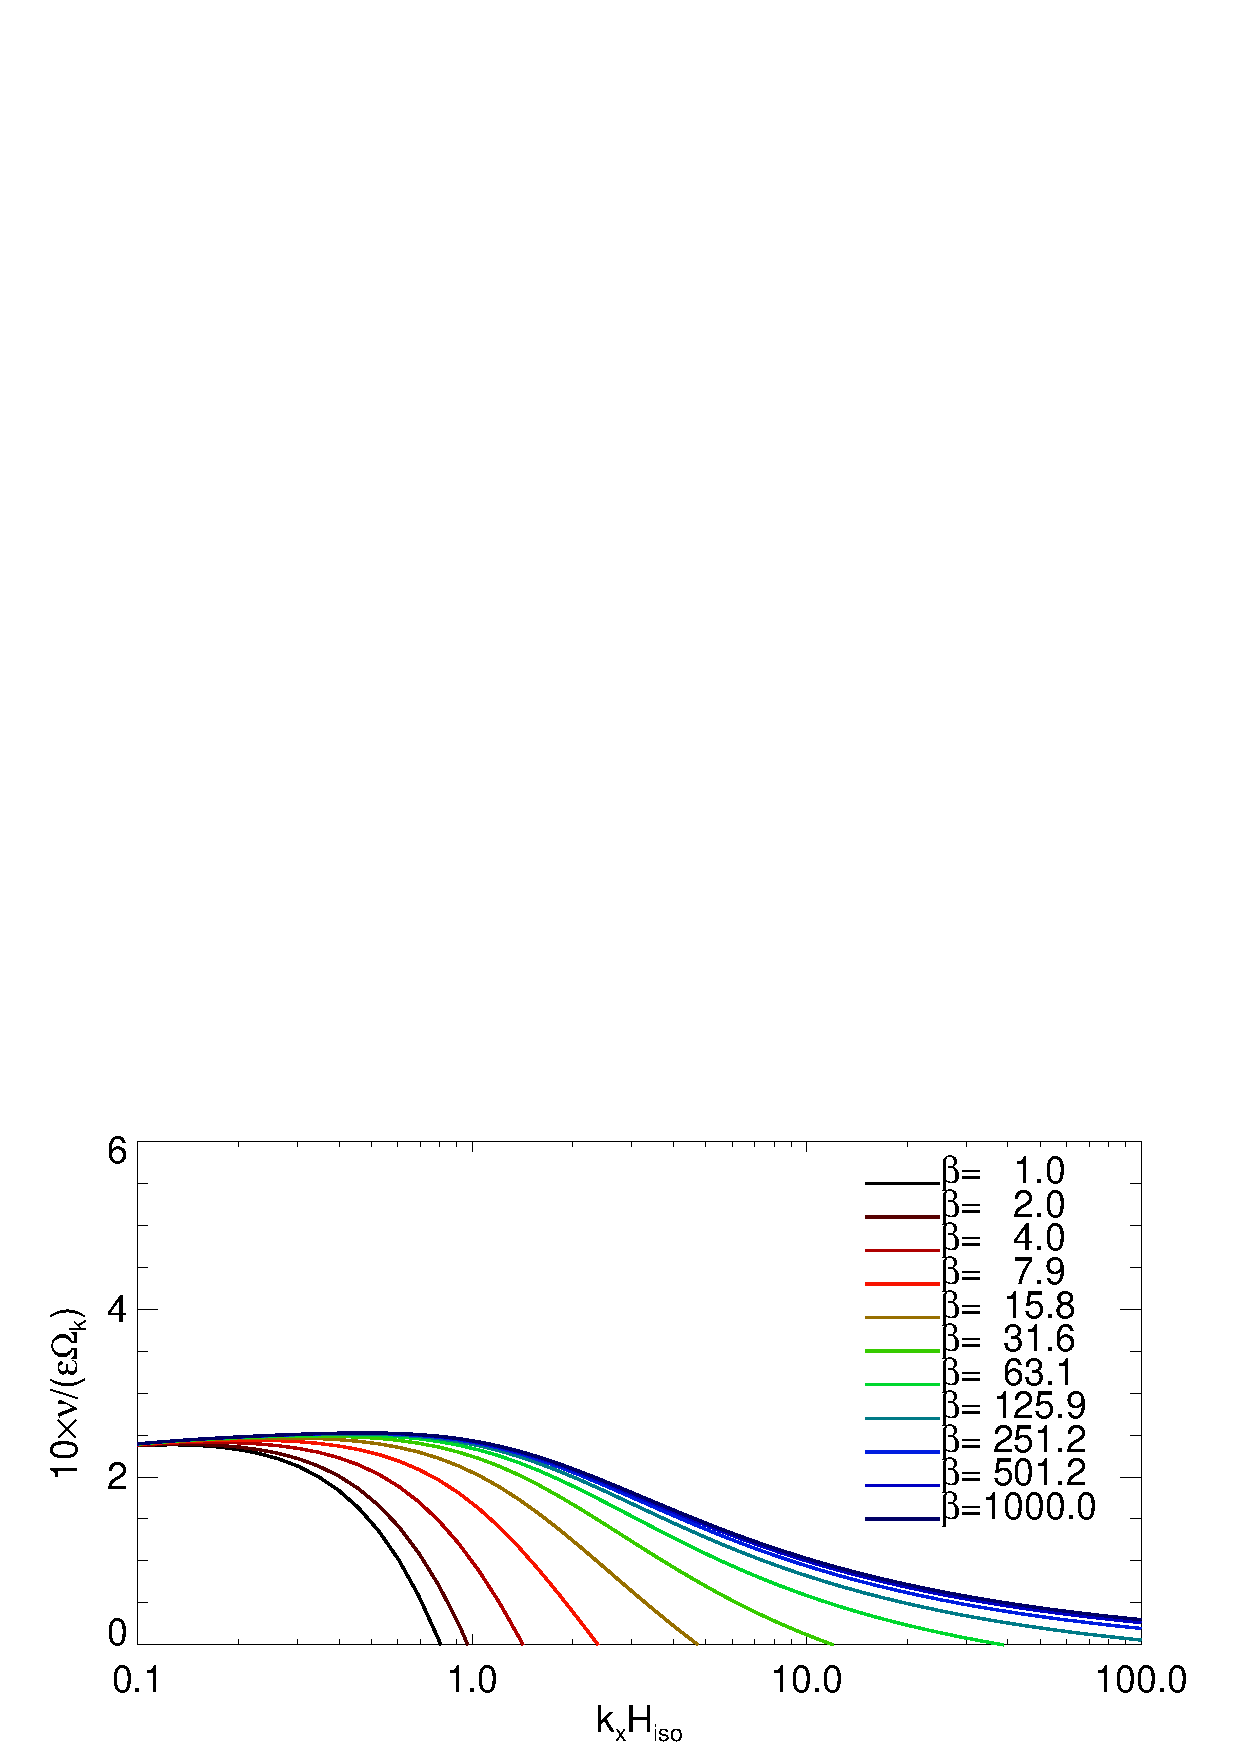
\includegraphics[width=\linewidth,clip=true,trim=0cm 0cm 0cm 1cm]{figures/compare_eigen_imag_bloop2}
  \caption{Growth rates of the fundamental VSI mode in
    nearly-vertically isothermal disks ($\Gamma=1.011$) with
    $\epsilon=0.05$ and $q=-1$, with thermal relaxation timescale
    $\beta$. The eigenfrequencies are calculated by numerically
    solving the full linear eigenvalue problem. \label{relax_growth_num}}   
\end{figure}   

We visualize the effect of thermal relaxation in 
Fig. \ref{relax_eigenW_num} by comparing the eigenfunction $W$ for
$\beta=0.01$ and $\beta=0.125$. The latter value is close to the critical
value beyond which the fundamental isothermal VSI is stabilized
(\S\ref{iso_vsi_beta_crit}).  Increasing $\beta$ restricts 
the region in which $W\sim z$ closer to the midplane, with oscillatory
behavior emerging at the boundaries, where buoyancy first becomes
important.  

\begin{figure}
  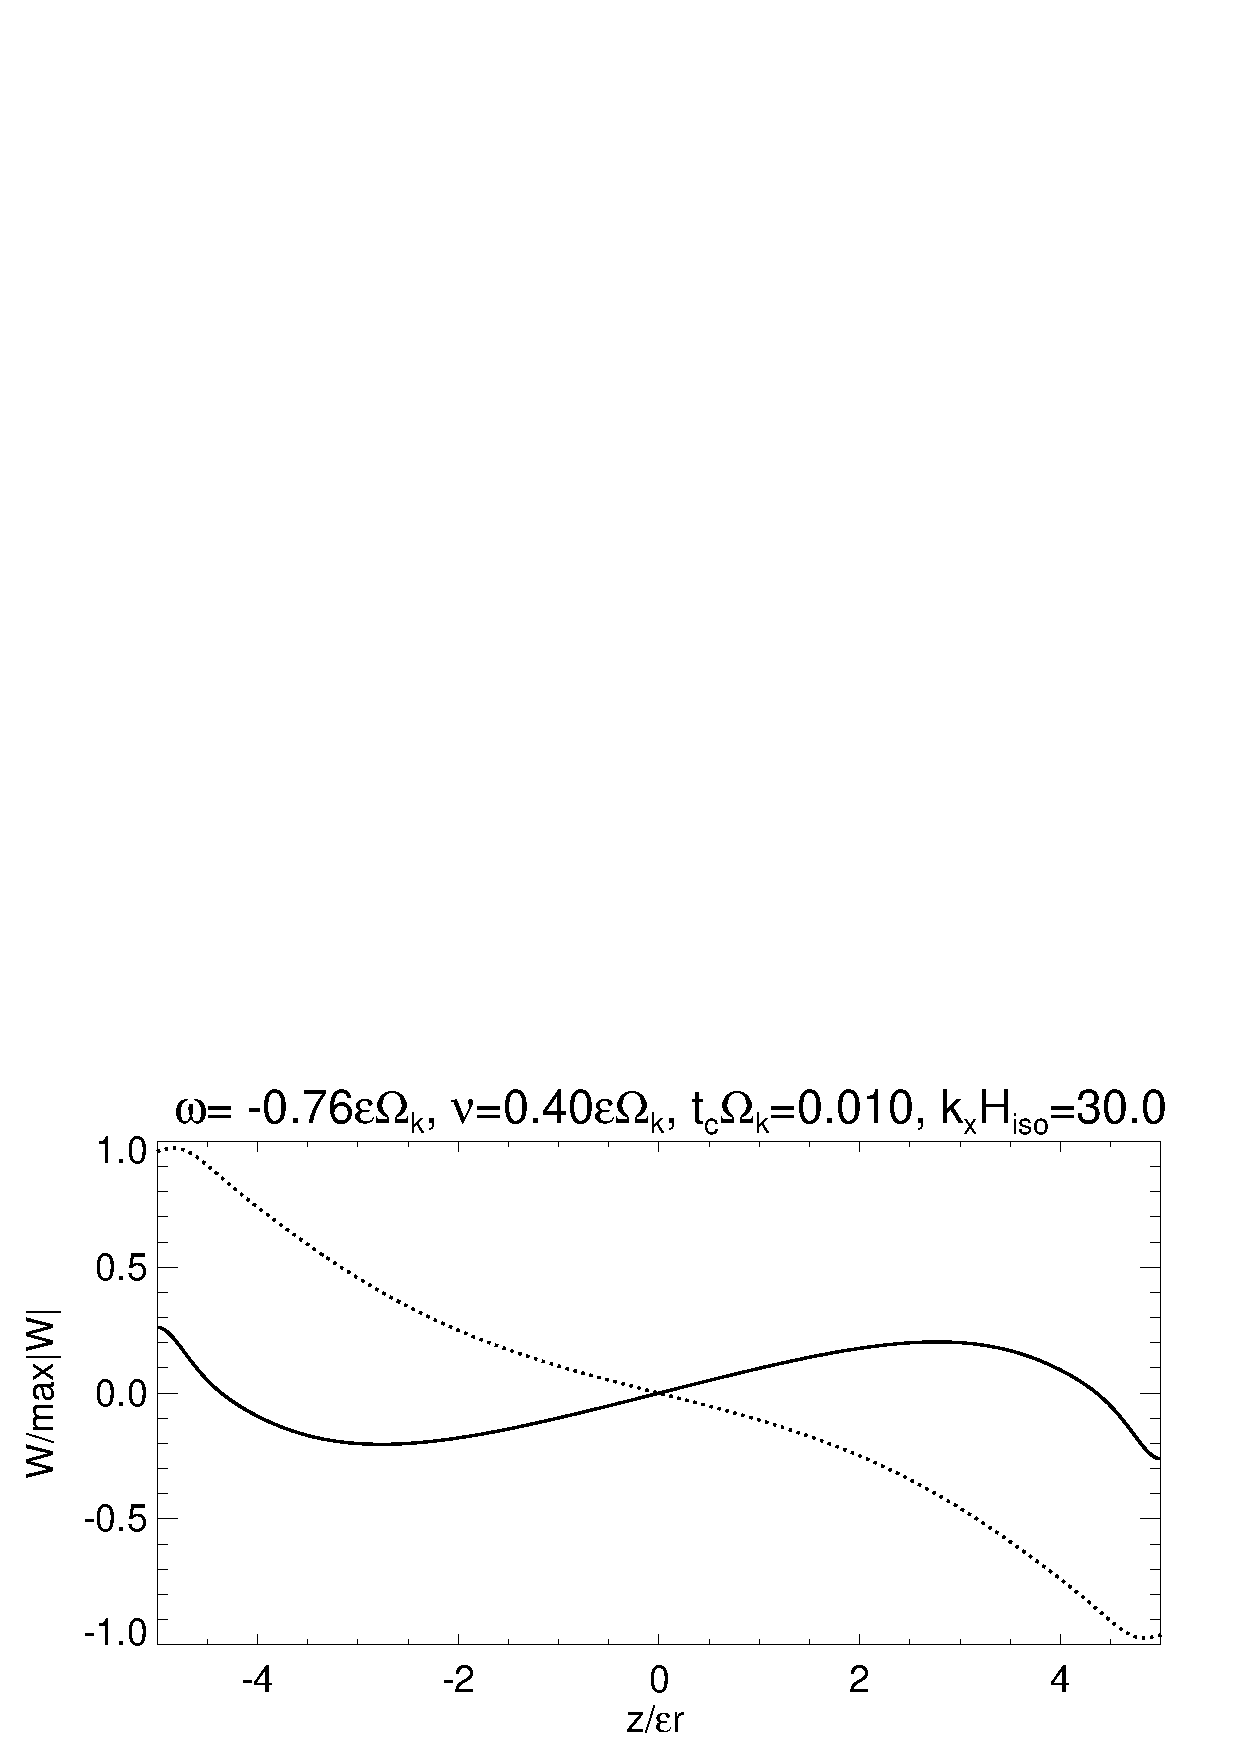
\includegraphics[width=\linewidth,clip=true,trim=0cm 1.75cm 0cm 0cm]{figures/eigenvectorW_beta0d01}
  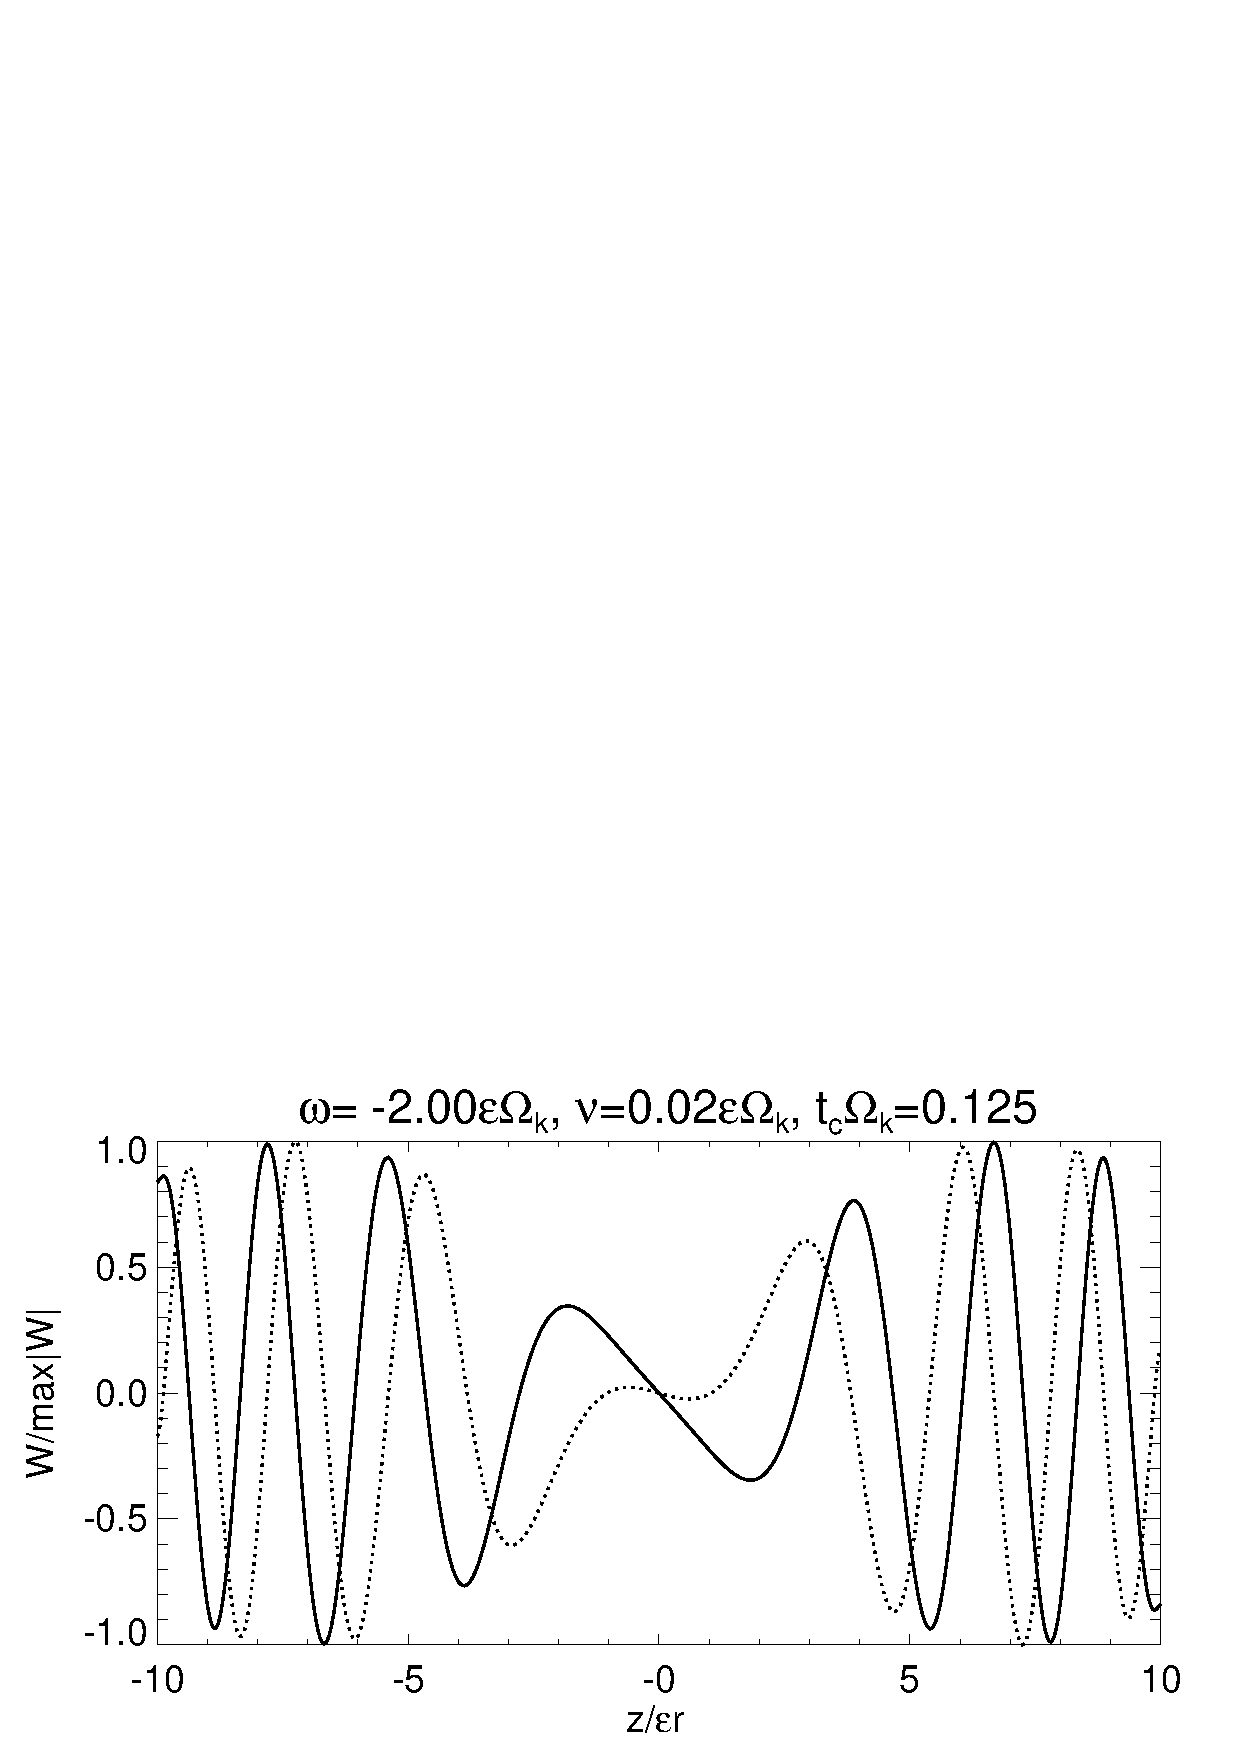
\includegraphics[width=\linewidth,clip=true,trim=0cm 0cm 0cm 0cm]{figures/eigenvectorW_beta0d125}
  \caption{Numerically-calculated eigenfunction of the fundamental VSI
    mode in a disk with dimensionless thermal relaxation timescale
    $\beta \equiv t_c\Omega_k = 0.01$ (top) and $0.125$ (bottom) for
    perturbations with a radial wavenumber $k_xH_\mathrm{iso}=10$. The
    real (imaginary) part of $W$ is plotted as the solid (dotted)
    line. Other disk parameters are
    $\epsilon=0.05$, $q=-1$ and $\gamma=1.4$.
    \label{relax_eigenW_num}}  
\end{figure}

%\citeauthor{nelson13} find a thermal relaxation timescale of
% $\beta\gtrsim 0.6$ stabilized the VSI for this disk model in non-linear
% hydrodynamic simulations. This is consistent with our numerical
% results.  

\subsection{Vertically non-isothermal disks}
We briefly consider vertically non-isothermal disks with
$\Gamma=1.4$. Other disk parameters are $p=0$, $q=-1.0$ and $\epsilon
= 0.05$. These are again chosen for comparison with \cite{nelson13}. 
In this case we set $\zmax\simeq2.2\epsilon r$, which is close to the
zero-density surface.     


\subsubsection{$N_z^2\equiv 0$}

Consider first the case $\gamma=1.4$ so that there is no vertical
entropy gradient. We plot in Fig. the growth rates for the
fundamental VSI for $\beta\in[10^{-2},10^{2}]$. We find growth rates
do not reach zero, implying the VSI operates regardless of the thermal
relaxation timescale if $\gamma=\Gamma$. This result is consistent
with \cite{nelson13}. 

We also note that growth rates for $\beta = 10^{-2}$ and
$\beta=10^{2}$ behave similarly. This is not surprising because
the linearized energy equation (Eq. \ref{lin_energy}) implies that 
\begin{align}
  W = \frac{\left(\Gamma^{-1} -
      \ii\hat{\sigma}\beta\right)}{\left(1-\ii\hat{\sigma}\beta\right)}
  Q \text{ for } \gamma\equiv \Gamma.   
\end{align}
Thus, $W \to Q/\Gamma$ as $\beta\to0$ and $W\to Q$ as
$\beta\to\infty$. Since $\Gamma=O(1)$, these two limits are expected
to produce qualitatively similar results.  

\begin{figure}
  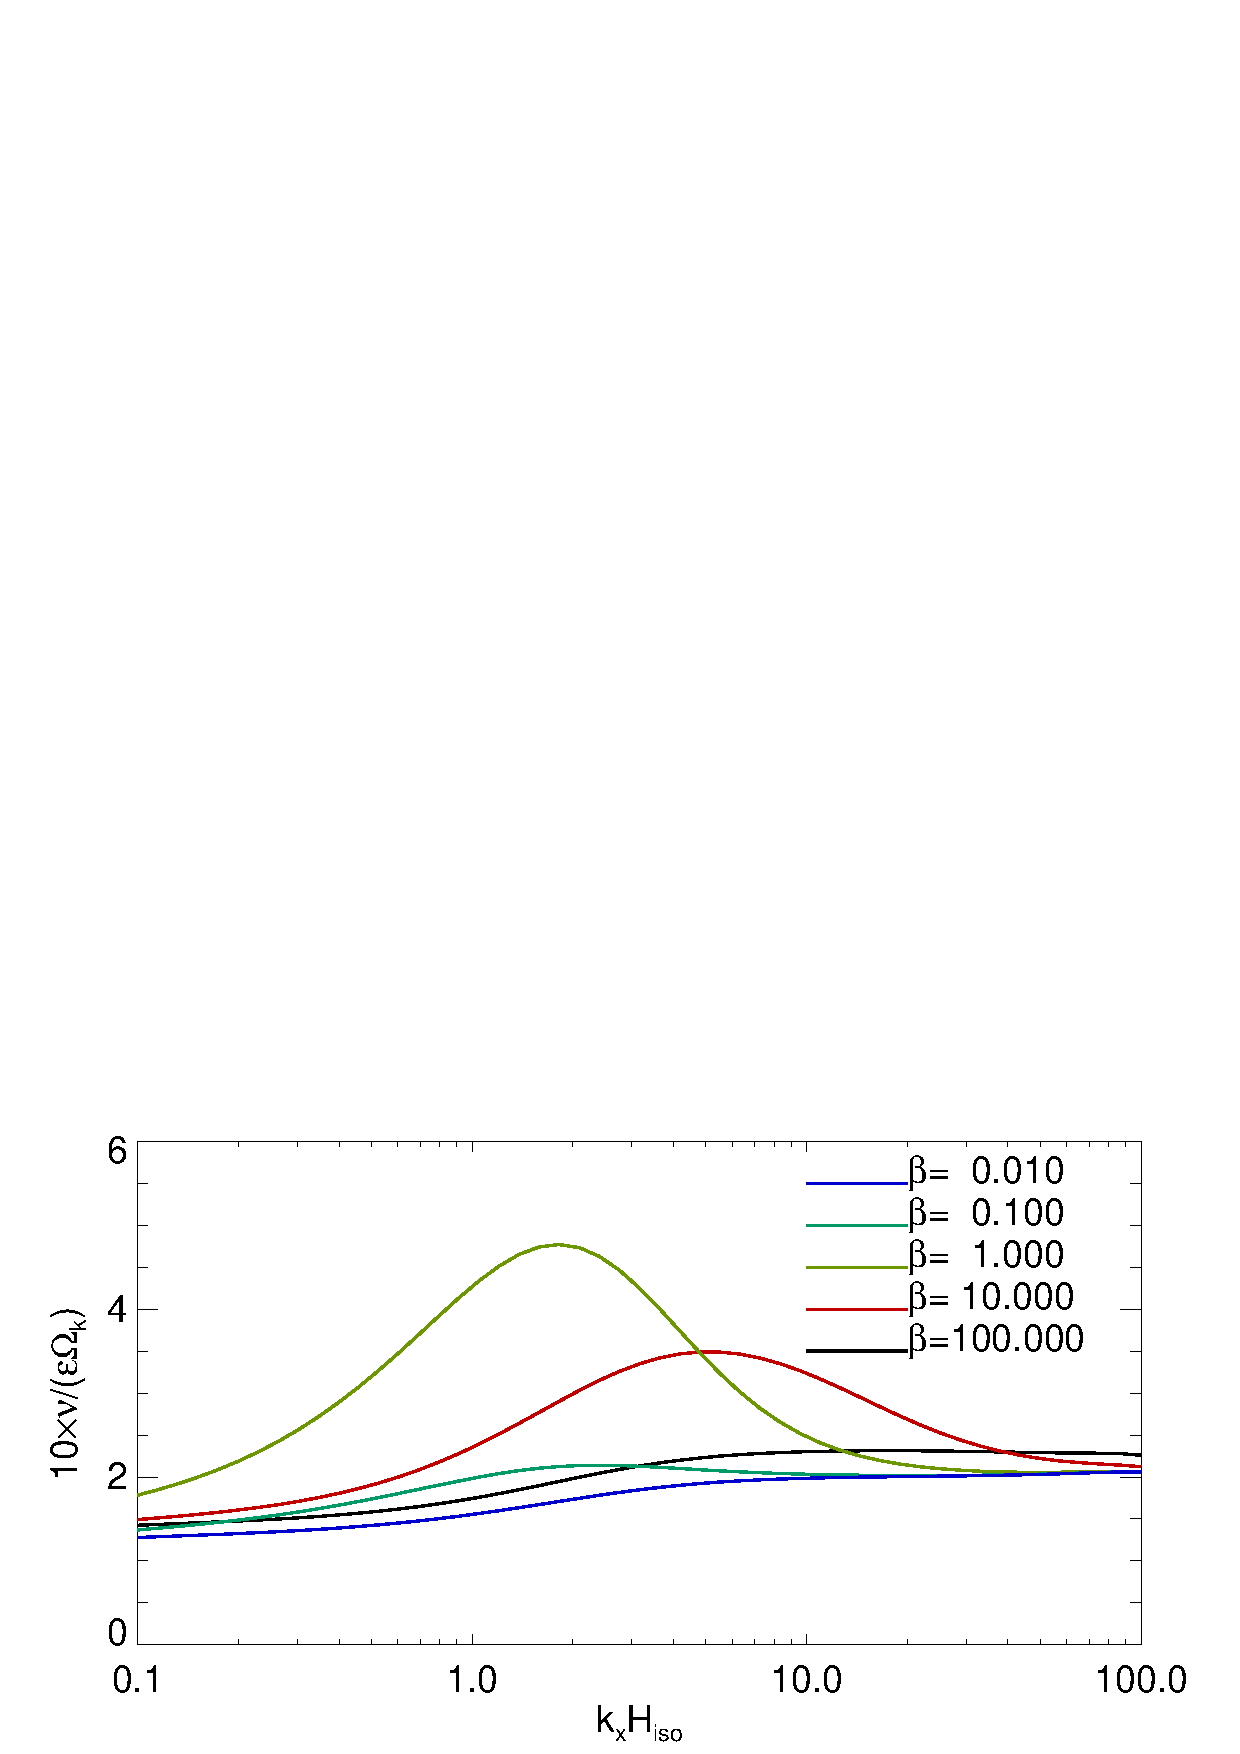
\includegraphics[width=\linewidth,clip=true,trim=0cm 0cm 0cm
  0cm]{figures/growth_vnoniso1} 
  \caption{Numerically-determined growth rates of the fundamental VSI
    mode in neutrally-buoyant, vertically non-isothermal disks
    ($\Gamma=\gamma=1.4$), with $p=0$, $q=-1$ and  $\epsilon=0.05$, for
    a range of thermal relaxation timescales
    $\beta$. \label{growth_vnoniso1}}     
\end{figure} 

Interestingly, Fig. \ref{growth_vnoniso1} show that growth rates
maximize for $\beta=O(1)$. However, all growth rates are similar to
order-of-magnitude for $0.1\lesssim\khat\lesssim 100$. 

\subsubsection{$N_z^2\geq0$}

%gamma = 2.0, Gamma = 1.4, vary bcool 

Finally, we introduce buoyancy in a vertically non-isothermal disk by
setting $\gamma=2$. This situation was not simulated in 
\cite{nelson13}, but is similar in spirit with vertically isothermal 
disks evolved with $\gamma>1$, as considered in the previous section. 

Fig. plots the growth rates for this case. The trend is
qualitatively similar to that for vertically isothermal disks with
$N_z^2\geq 0$ (Fig. \ref{relax_growth_num}), namely growth rates reach
zero at finite $\khat$. 

  